\section{Meshes}
\label{sec:meshes}

Meshes are fundamental in computer graphics, imaging
and data analysis. In this section, we share applications
where the Gauss-Bonnet theorem is used to increase
the quality of meshes and decrease the size.


\subsection{Removing Noise From A Scanned Object}

Meshes that are obtained by scanning real objects contain noise.
Most meshes that are generated by scanning require a complete
remeshing \cite{remeshing-2003}.
As a first step in remeshing, the curvature at each
vertex needs to be estimated.

In \cite{mmsb-2003}, Meyer et al., define the gaussian curvature operator
to estimate the curvature at each vertex. Their operator is 
based on a simple application of the Gauss-Bonnet theorem.
The central idea is to cut a disk around each vertex that does not contain
any other vertices. Then, all Gaussian curvature in the removed
disk is occurs at the vertex of interest.

We associate an area around each vertex$v$. 
For each triangle incident to $v$, if the interior 
angle at $v$ is non-obtuse, mark the circumcenter of the triangle
and if the interior angle is obtuse, make the mid point of the edge
opposite of $v$. See \figref{mixed-area} for an illustration.
Denote the area of this polygon by $A_m.$


\begin{figure}[htb]
\centering
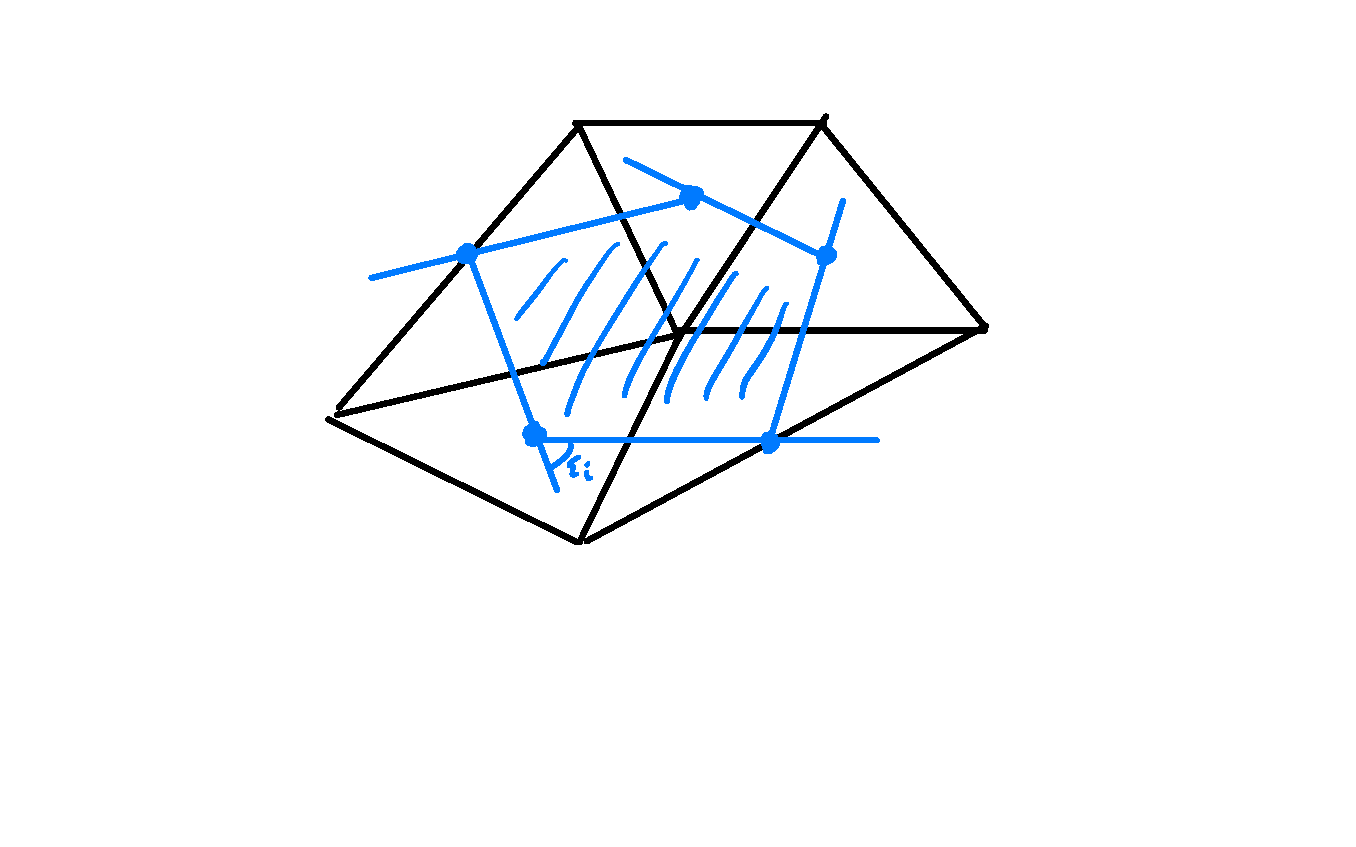
\includegraphics[width=.3\textwidth]{meshes/mixed-area}
\caption{The area $A_m$ associated with a vertex $v$.}
\label{fig:mixed-area}
\end{figure}


Then, since we are considering a closed two-disk $A$ we have $\chi(A)=1$.
Let $F_v$ denote the number of faces incident to $v$, 
then by the Gauss-Bonnet theorem we have

$$\int \int_{A_m}K dA +\sum_i^{F_v} \epsilon_i=2\pi$$
where the sum is over the faces incident to $v$.
The Gaussian curvature operator at a vertex $v$ is defined
to be
$$K(v)=\left( 2\pi -\sum_i^{F_v}\epsilon_i\right)/ A_m.$$

The experiments in \cite{mmsb-2003} found that the average
percent error did not exceed $1.3\%$ when using this operator.

\subsection{Triangulating Noncovex Polytopes}

Often, the mesh representing
an object contains more triangles than is necessary. One then wishes to
discard triangles without altering the geometry of the object \cite{simplify-mesh-1999}.
In three dimensions, meshes consist of tetrahedra. 
In \cite{triangulating-polytope-1990}, Chazell and Palios give an
algorithm to triangulate a nonconvex three-dimensional polytope.
The algorithm runs in $O(n+r^2)$ tetrahedra where $n$ is the number
of vertices and $r$ is the number of reflex edges.

A  \EMPH{polyhedron of genus $g$} is a combinatorial three-manifold with 
boundary homeomorphic to a $g$ holed torus.
For a genus $g$ polyhedron, it is natural to ask if one can 
triangulate the manifold with fewer than $O(n+r^2)$ tetrahedra.


Chazelle and Shouraboura us the 
 Gauss-Bonnet theorem shows that, any polyhedron
can be triangulated with $O(n+r^2)$ tetrahedra, regardless  of 
the genus! Moreover, this bound is tight \cite{tetra-bounds-c-s-1994}.
Here is their application.

Let $P$ be a a simple polytope. An edge $e$ in $P$ is
\EMPH{reflex} the interior angle formed by its two incident faces
is greater than $\pi$.
A vertex is reflex is it is incident to a reflex edge.

\begin{theorem}[Reflex Angles]\label{thm:reflex}

Any polyhedron of genus $g$ must have 
at least $g-1$ reflex dihedral angles. 

\end{theorem}

From \thmref{reflex}, it follows that any polyhedron
with $n$ vertices and $r$ reflex angles
can be triangulated with $O(n+r^2)$ tetrahedra 
and the bound is tight. Notice that this result is independent
of the genus.

Let $T$ be a tetrahedra, here, the curvature at a vertex $k_v$ is defined to
be the sum of the angle defect.
The Euler characteristic of a polyhedron is determined by the genus,
$\chi=2-2g$.
Polyhedra do not have a 1-dimensional boundary, 
so, the Gauss-Bonnet theorem,
$$\sum_vk_v=2\pi (2-2g).$$

We show that
$$g\leq r+1.$$ 
Then, \thmref{reflex} will be a consequence of the following
lemma,

\begin{lemma}\label{lem:reflex-edge}
The number of reflex edges  incident to a vertex $v$  is at least $-k_v.$
\end{lemma}

\begin{proof}
Project the faces incident to $v$ onto a 2-sphere centered at $v$
to obtain a ``polygon" $P$on the sphere made  of great circles.
An edge in $T$ is reflex if and only if it gives  a reflex angle on $P$.

Let $L$ be the length of the curve and $R$ is  number of reflex  angles.
Then

\begin{equation} \label{eqn:length-reflex}
L\leq 2\pi (R+1)
\end{equation}
Note, if $R$ is zero then \eqnref{length-reflex}
tells us that the curvature at a convex point is non-negative.

If $R\neq 0$, we draw arcs of great circles from each reflex point
along the bisector of its reflex angle, and thus decompose the unit sphere
into at most $R+1$ convex regions. (Convex here means
great circles are contained in the region).
Apply the $R=0$ case $R+1$ times.

\end{proof}



